% TITLE: Marjum Pass 2026-07: the vector E-field beam from the transmitter raster
% AUTHORS: EIGSEP Team
% TAGS: Beam, Polarization, Transmitter, Marjum 2026-07
% SUMMARY: Box-air's complex vector beam solved per pixel from the 07-17 transmitter raster's cross-correlation, with no HFSS input to the solve; agreement with HFSS, the role of the azimuth handedness and axle tilt, and what limits the cross-polar components.
\documentclass{aastex631}

\usepackage{amsmath}
\newcommand{\mapNpixA}{3833}
\newcommand{\mapNpixB}{3284}
\newcommand{\mapNpixC}{3460}
\newcommand{\mapRmsDbA}{0.42}
\newcommand{\mapRmsDbB}{0.49}
\newcommand{\mapRmsDbC}{0.72}
\newcommand{\medPowerL}{0.981}
\newcommand{\medPowerLzero}{0.976}
\newcommand{\medPowerR}{0.977}
\newcommand{\medXL}{0.986}
\newcommand{\medXLzero}{0.985}
\newcommand{\medXR}{0.985}
\newcommand{\medYL}{0.985}
\newcommand{\medYLzero}{0.944}
\newcommand{\medYR}{0.958}
\newcommand{\medZL}{0.983}
\newcommand{\medZLzero}{0.976}
\newcommand{\medZR}{0.981}
\newcommand{\nTeeth}{29}
\newcommand{\tiltHfssL}{+6}
\newcommand{\tiltHfssR}{-7}


\newcommand{\vu}{\mathbf{u}}
\newcommand{\vE}{\mathbf{E}}
\newcommand{\rhat}{\hat{\mathbf{r}}}

\begin{document}

\title{Marjum Pass 2026-07: the vector E-field beam from the transmitter raster}

\author{EIGSEP Team}
\affiliation{Department of Astronomy, University of California Berkeley, Berkeley, CA 94720, USA}
\affiliation{Radio Astronomy Laboratory, University of California Berkeley, Berkeley, CA 94720, USA}

\begin{abstract}
We recover box-air's complex vector beam, not only its power pattern, from the 07-17 transmitter raster. Each
sky pixel gets a complex 3-vector $\vu$, solved from the box-air $\times$ box-gnd cross-correlation on the
transmitter's two orthogonal arms. HFSS does not enter the solve. With the left-handed azimuth and the
$+4.7^\circ$ elevation-axle tilt of living memo 003, the median per-tooth correlation with HFSS over
\nTeeth\ teeth (171.9--226.6\,MHz) is \medXL\ ($|u_x|^2$), \medYL\ ($|u_y|^2$), \medZL\ ($|u_z|^2$) and
\medPowerL\ (total power). Without the tilt, the cross-polar $y$ component drops to \medYLzero. Where $y$
and $z$ still differ from HFSS, deep in their nulls, the difference mostly repeats between independent passes
over the same pixel, so it is not noise. This memo describes the inputs, the per-pixel solve, the tests, a
per-dwell common phase in the cross-correlation whose cause is open, and what remains.
\end{abstract}

\section{Summary}
\begin{itemize}
\item \textbf{Data:} \nTeeth\ transmitter teeth from 171.9 to 226.6\,MHz, 6810 integrations of 0.54\,s over
  20:26:00--21:28:40\,UTC on 07-17, cross-correlation only.
\item \textbf{The solve agrees with HFSS} to a median \medXL, \medYL, \medZL\ and \medPowerL\ ($x$, $y$, $z$,
  total power; Fig.~\ref{fig:scores}). Sky maps agree to \mapRmsDbA--\mapRmsDbC\,dB (power-weighted rms;
  Figs.~\ref{fig:mapsA}--\ref{fig:mapsC}).
\item \textbf{The mount is taken from the living memos, not fitted here:} memo 002's v0005 positions, and memo
  003's left-handed azimuth, azimuth zero, elevation zero and axle tilt (\S\ref{sec:geometry}).
\item \textbf{The axle tilt matters most for $y$.} Adding the $+4.7^\circ$ tilt raises $y$'s median correlation
  from \medYLzero\ to \medYL. Before the azimuth handedness was settled, the right-handed solve gave \medYR.
\item \textbf{Pointing was the first big lever.} The production pointing table lifted $y$ from 0.68 to 0.93 over
  the potentiometer azimuth, which had slipped by up to $27^\circ$ (\S\ref{sec:geometry}).
\item \textbf{The worst cells were extrapolated fills.} Requiring every interleave fill to lie between measured
  teeth of its arm removed them (\S\ref{sec:data}).
\item \textbf{At the nulls the remaining error is not noise:} 71--74\% of the variance against HFSS repeats
  between dwells (\S\ref{sec:nulls}). It is small in total power.
\item \textbf{A common cross-correlation phase jumps between dwells}, identically in every tooth. A
  self-calibration removes it but calibrates only 62\% of the integrations, so it is not used (\S\ref{sec:phase}).
  The jumps grow while the box rocks along the axle; their cause is open (\S\ref{sec:jumps}).
\end{itemize}

\section{Why a vector beam} \label{sec:why}
A power beam cannot separate pointing, polarization and beam errors; a complex vector beam can, because each
acts differently on $\vu$. The raster gives more than power. The transmitter radiates on two orthogonal arms on
alternate comb teeth, and the cross-correlation with the ground antenna keeps each tooth's phase. One integration
therefore measures two complex projections of the beam,
\begin{equation}
V_x = \vE_1\cdot\vu, \qquad V_y = g\,\vE_2\cdot\vu, \label{eq:model}
\end{equation}
where $\vE_1$, $\vE_2$ are the transmitter arms' fields in the antenna's body frame (the frame of the HFSS beam)
and $g$ is one complex arm ratio per tooth. A Mueller or Stokes treatment does not avoid the need for this phase;
it only adds partial polarization, which nothing here calls for.

\section{Data and inputs} \label{sec:data}
The input is the 07-17 raster (memo 003). Elevation turns continuously at about $5.2^\circ\,\mathrm{s}^{-1}$
while azimuth steps $5^\circ$ once per 70.8\,s revolution, with the antenna at the 91\,m configuration and the
transmitter $3.7^\circ$ from nadir. The reduction (\texttt{eigsep\_data.beam\_mapping.vector\_beam.reduce\_cross}):
\begin{enumerate}
\item \textbf{Teeth.} Box-air $\times$ box-gnd cross spectra on every 8th channel, arms alternating.
\item \textbf{Comb subtraction} against a three-point local baseline. (The autos use a full DPSS bandpass;
  whether the difference matters is open.)
\item \textbf{Trust mask.} FM (87--108\,MHz) and tones above 230\,MHz are untrusted. A flagged tone of an arm's
  own stays NaN.
\item \textbf{Interleave fill.} Each tooth measures one arm; the other arm's value there is never measured. A
  fixed 91.65\,ns cable delay is removed, each arm's real and imaginary parts are fitted with 23 DPSS modes over
  its $\sim$27--31 trusted teeth, the fit is interpolated to the slot between two same-arm teeth (1.95\,MHz
  either side), and the delay is restored. After the delay is removed, the phase moves a median 5--8$^\circ$
  between same-arm teeth, and a measured tooth predicted from neighbours twice as far away is good to
  3--5$^\circ$ and 1--2\% (median). About 1\% of steps exceed $110^\circ$, presumably near nulls.
\item \textbf{Bracketed fills only.} A fill counts only if measured teeth of its arm lie on both sides.
  Unbracketed fills were extrapolations up to $\sim10^4$ times the median and caused every absurd cell. The
  rule costs a median 9\% of pixels and loses the last tooth.
\item \textbf{Rows:} those \texttt{fit\_beam.py} uses, minus bad times. Flagged values stay NaN throughout;
  nothing is filled in their place.
\end{enumerate}

\section{The solve} \label{sec:solve}
Each pixel's $\vu$ is a least-squares solve over the integrations that land in it. There is no smoothing across
pixels or frequency, and nothing is produced for an unvisited pixel. Each integration $i$ gives three rows, the
two arm projections and a transversality row:
\begin{equation}
\begin{pmatrix} \vE_{1,i}^{\mathsf T} \\ \vE_{2,i}^{\mathsf T} \\ \rhat_i^{\mathsf T} \end{pmatrix} \vu_p =
\begin{pmatrix} V_{x,i} \\ V_{y,i}/g \\ 0 \end{pmatrix}. \label{eq:solve}
\end{equation}
Here $\rhat_i$ is the unit vector from the antenna toward the transmitter at integration $i$, in the body frame:
the direction of the pixel being solved, which differs from pixel to pixel as the antenna rolls. It is not a
fixed axis. The third row says only that the far-field beam is transverse to the incoming direction. It does not
force $u_z=0$, except at the boresight pole where $\rhat=\hat{\mathbf z}$. In spherical components
$u_z=-\sin\theta\,E_\theta$, so $|u_z|^2$ is dark near both poles by geometry alone. $\vE_{1,i}$ and $\vE_{2,i}$
are also projected transverse to $\rhat_i$. The phase-centre path (memo 003 \S7) is $\rhat\cdot\mathbf r_{\rm pc}$,
fixed for a body-frame direction, so it is a per-pixel phase absorbed into $\vu$; $\vu$ is referenced to the
elevation axle, not to HFSS's origin.

\textit{Caveat.} Each integration uses its own continuous $\rhat_i$, not the pixel centre, but $\vu_p$ is one
vector per pixel. With several visits it is asked to be perpendicular to directions up to $\sim1.8^\circ$ apart,
and least squares balances that against the data rows. The zero row has unit weight while the data rows are in
correlator units, so with several visits the strength of the transversality constraint depends on the data's
scale. With one integration (87\% of pixels) the system is square and the constraint is exact.

The rows are independent (one integration's condition number is $\approx2.9$), so one integration determines
$\vu$. Pixels enter if the stacked condition number is at most 30.
\begin{itemize}
\item \textbf{Pixels and dwells.} HEALPix $N_{\rm side}=32$ ($\approx1.8^\circ$) in the body frame. Elevation
  moves $\approx2.8^\circ$ per integration, so one pass over a pixel (a \emph{dwell}) puts one integration in it
  97\% of the time. Of the 5343 visited pixels, 87\% are seen in one dwell, 11\% in two and 3\% in three or more.
  Only the multi-dwell pixels can test the solve and fit $g$.
\item \textbf{Closure $g$.} One complex arm ratio per tooth, fitted with no beam model. A pixel with $n\ge3$ visits
  gives $3n$ equations for 3 unknowns, and the residual collapses only when $g$ and the geometry are right.
  $g$ is refitted for every geometry: its phase flips by $\sim180^\circ$ with the azimuth handedness.
\item \textbf{Geometry.} $\vE_1$, $\vE_2$ and $\rhat$ come from the production model
  (\texttt{TxGeometryModel}), so the solve shares one pointing convention with \texttt{JointBeamFit}.
\end{itemize}

\section{Geometry and pointing} \label{sec:geometry}
The left-handed azimuth is implemented as pointing table v5 does it: the right-handed model fed $-$az. The mount
values are the published ones, and none is fitted here:
\begin{itemize}
\item positions: memo 002's v0005 posterior means (camera poses and the joint MCMC);
\item handedness: left-handed about the boresight (memo 003 \S5.1, from the azimuth IMU and two photographs);
\item azimuth zero $+15.8^\circ$ from the highline and arm-0 polarization angle $\alpha\approx8^\circ$
  (memo 003 \S5.2);
\item elevation zero $+0.05^\circ$ and elevation-axle tilt $+4.7^\circ$ (WNW end low), from the v0016 beam fit
  (memo 003 \S6).
\end{itemize}
The v0016 fit's other geometry corrections are not applied here.

Table~\ref{tab:history} records how the inputs moved the result before the handedness was settled, under the
right-handed azimuth and memo 005's v0013 corrections. The potentiometer azimuth had slipped by up to $27^\circ$
against the platform (memo 003 \S4), which is a polarization rotation and showed up mostly in $y$.

\begin{table}[h]
\centering
\caption{Median correlation with HFSS per tooth through the inputs' history (right-handed azimuth, v0013
  geometry). The first row reproduces the September 2026 results to $6\times10^{-16}$, so the gains come from
  the inputs.}
\label{tab:history}
\begin{tabular}{llccc}
\hline
stage & pointing and geometry & $y$ & $z$ & power \\
\hline
September 2026 & potentiometer azimuth, September fit & 0.677 & 0.846 & 0.934 \\
pointing table & pointing table v3, v0013 corrections & 0.930 & 0.907 & 0.954 \\
+ bracketed fill & same & 0.958 & 0.981 & 0.977 \\
\hline
\end{tabular}
\end{table}

A constant azimuth offset and a constant polarization angle are exactly degenerate with a rotated beam in the
HFSS-free consistency test (scans flat to $10^{-4}$), so the data alone cannot fix them; the published values
from the polarization fit of memo 003 are used.

\section{Comparison with HFSS} \label{sec:hfss}
Figure~\ref{fig:scores} gives the per-tooth correlation of each component with HFSS under three mounts: the
right-handed v0013 geometry used before the handedness was settled, the left-handed mount with no tilt, and the
left-handed mount with the $+4.7^\circ$ tilt. Figures~\ref{fig:mapsA}--\ref{fig:mapsC} show the components and
total gain at three teeth for the last.

The recovered beam has an unknown overall scale. The correlations align it to HFSS by one least-squares complex
factor per tooth and do not depend on it. The maps instead scale the recovered power by one real least-squares
factor per tooth. A single complex factor understates the amplitude by 6--8\,dB, because each pixel's phase
relative to HFSS differs (the phase-centre path and the per-dwell phase jumps), which washes out the complex
overlap. Nothing else from HFSS enters. Unsampled pixels are grey; most of the sky is sampled only along the
raster's tracks.

\textit{Coverage.} The auto-correlation power method on the same integrations covers 3645 pixels at 199.2\,MHz
and 5290 at 222.7\,MHz, against 3317 and 3518 with valid cross data after the bracketed-fill rule, of which the
solve keeps 3284 and 3460. The bracketed-fill rule and the cross-tone flags remove more integrations than the
auto flags, most of all above $\sim$210\,MHz. At 175.8\,MHz the auto is chronically contaminated by RFI and
covers only 46 pixels, while the cross is clean.

\begin{figure*}[t]
\centering
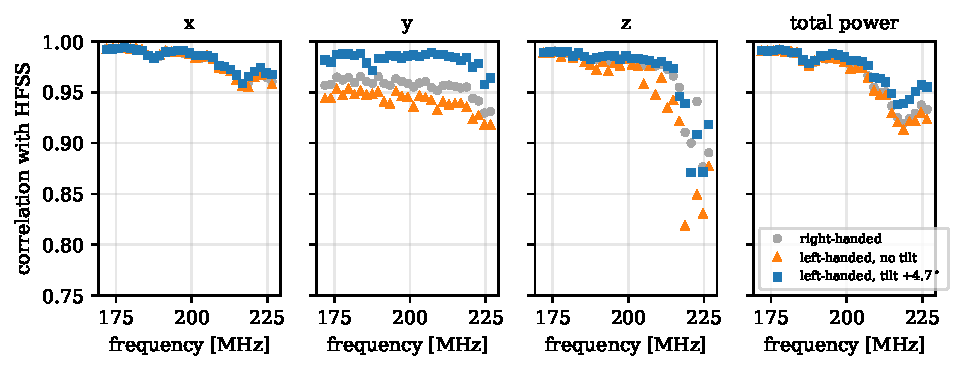
\includegraphics[width=\textwidth]{figures/scores_vs_freq.pdf}
\caption{Correlation with HFSS per tooth of $|u_x|^2$, $|u_y|^2$, $|u_z|^2$ and total power. Grey: right-handed,
  v0013 geometry. Orange: left-handed, no tilt. Blue: left-handed, $+4.7^\circ$ axle tilt (the maps). Medians
  ($x$, $y$, $z$, total): right-handed \medXR, \medYR, \medZR, \medPowerR; left-handed untilted \medXLzero,
  \medYLzero, \medZLzero, \medPowerLzero; left-handed tilted \medXL, \medYL, \medZL, \medPowerL. Without the
  tilt the left-handed mount loses $y$ and, above $\sim$215\,MHz, $z$.}
\label{fig:scores}
\end{figure*}

\begin{figure*}[p]
\centering
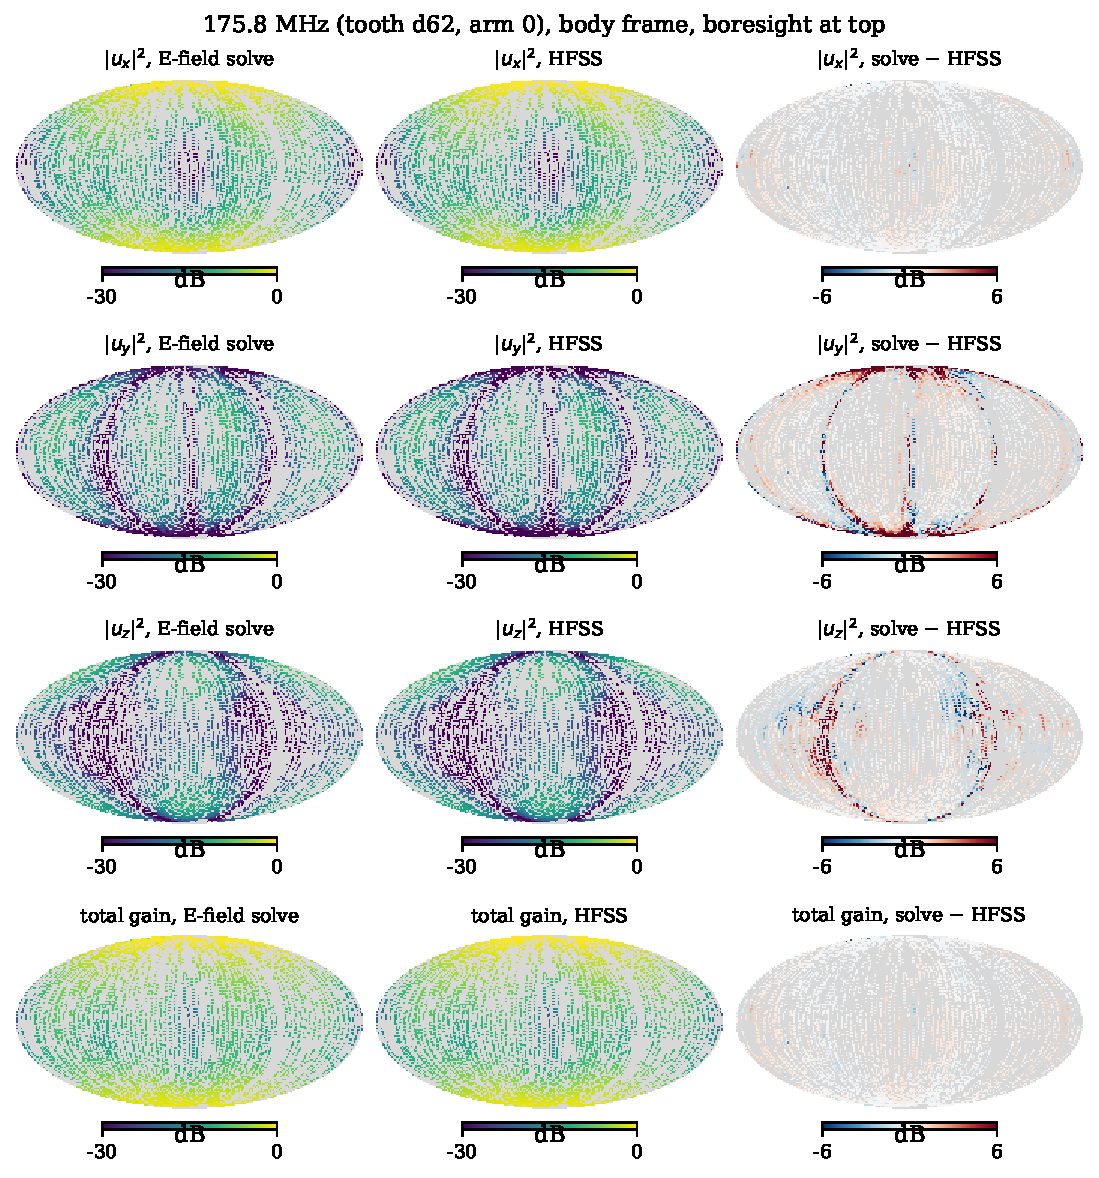
\includegraphics[width=0.92\textwidth]{figures/maps_d62.pdf}
\caption{175.8\,MHz. Rows: $|u_x|^2$, $|u_y|^2$, $|u_z|^2$ and total gain, in dB relative to HFSS's peak total
  gain on the sampled pixels. Columns: E-field solve, HFSS, and their difference. Body frame, Mollweide,
  boresight at the top; left-handed mount with the axle tilt; \mapNpixA\ pixels solved; power-weighted rms
  difference of the total \mapRmsDbA\,dB.}
\label{fig:mapsA}
\end{figure*}

\begin{figure*}[p]
\centering
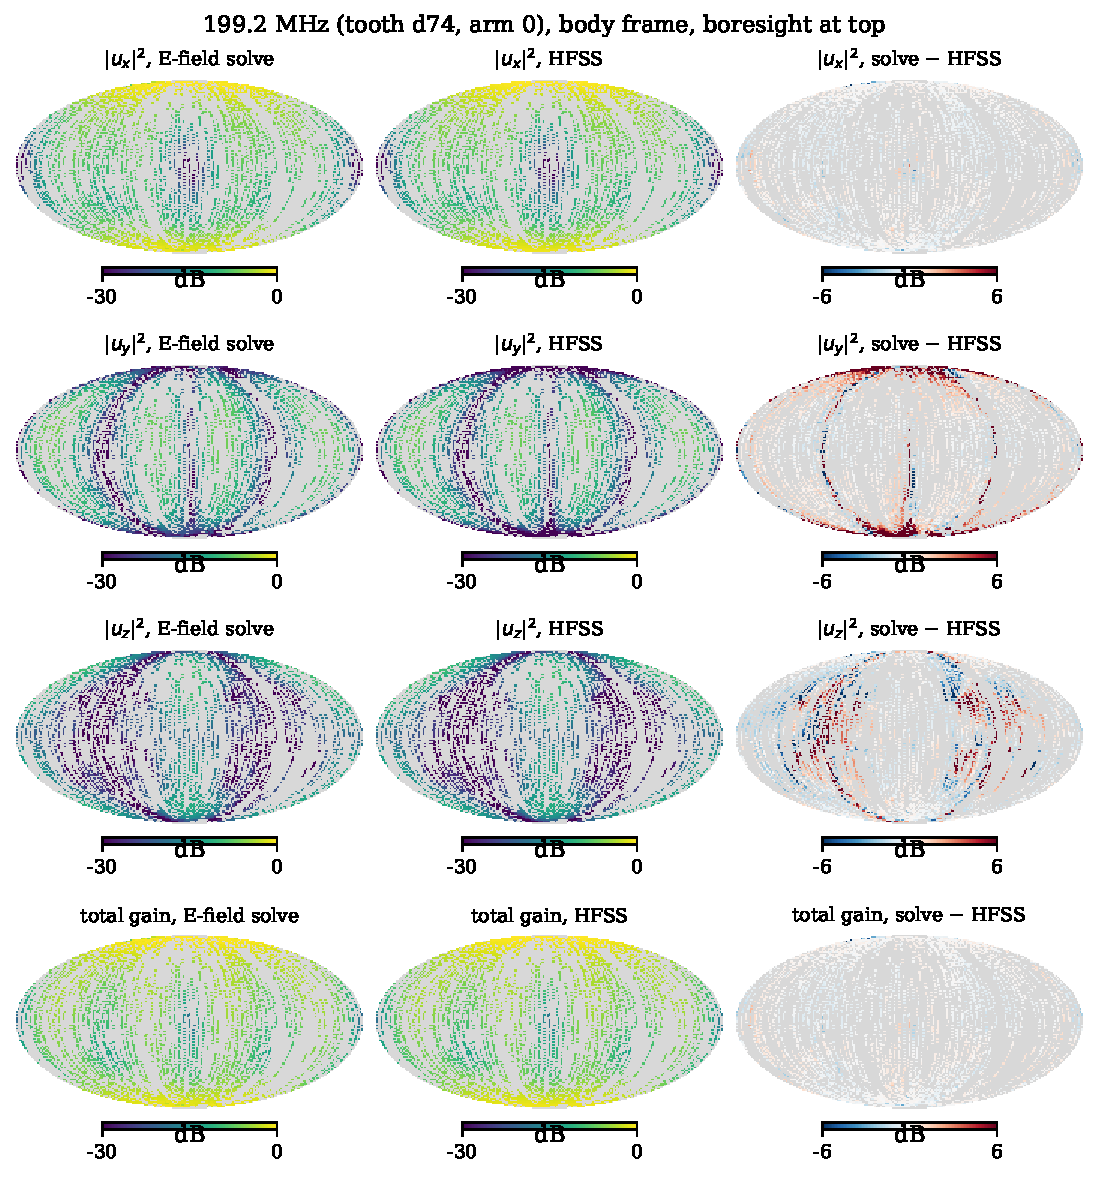
\includegraphics[width=0.92\textwidth]{figures/maps_d74.pdf}
\caption{As Fig.~\ref{fig:mapsA} at 199.2\,MHz; \mapNpixB\ pixels; rms difference \mapRmsDbB\,dB.}
\label{fig:mapsB}
\end{figure*}

\begin{figure*}[p]
\centering
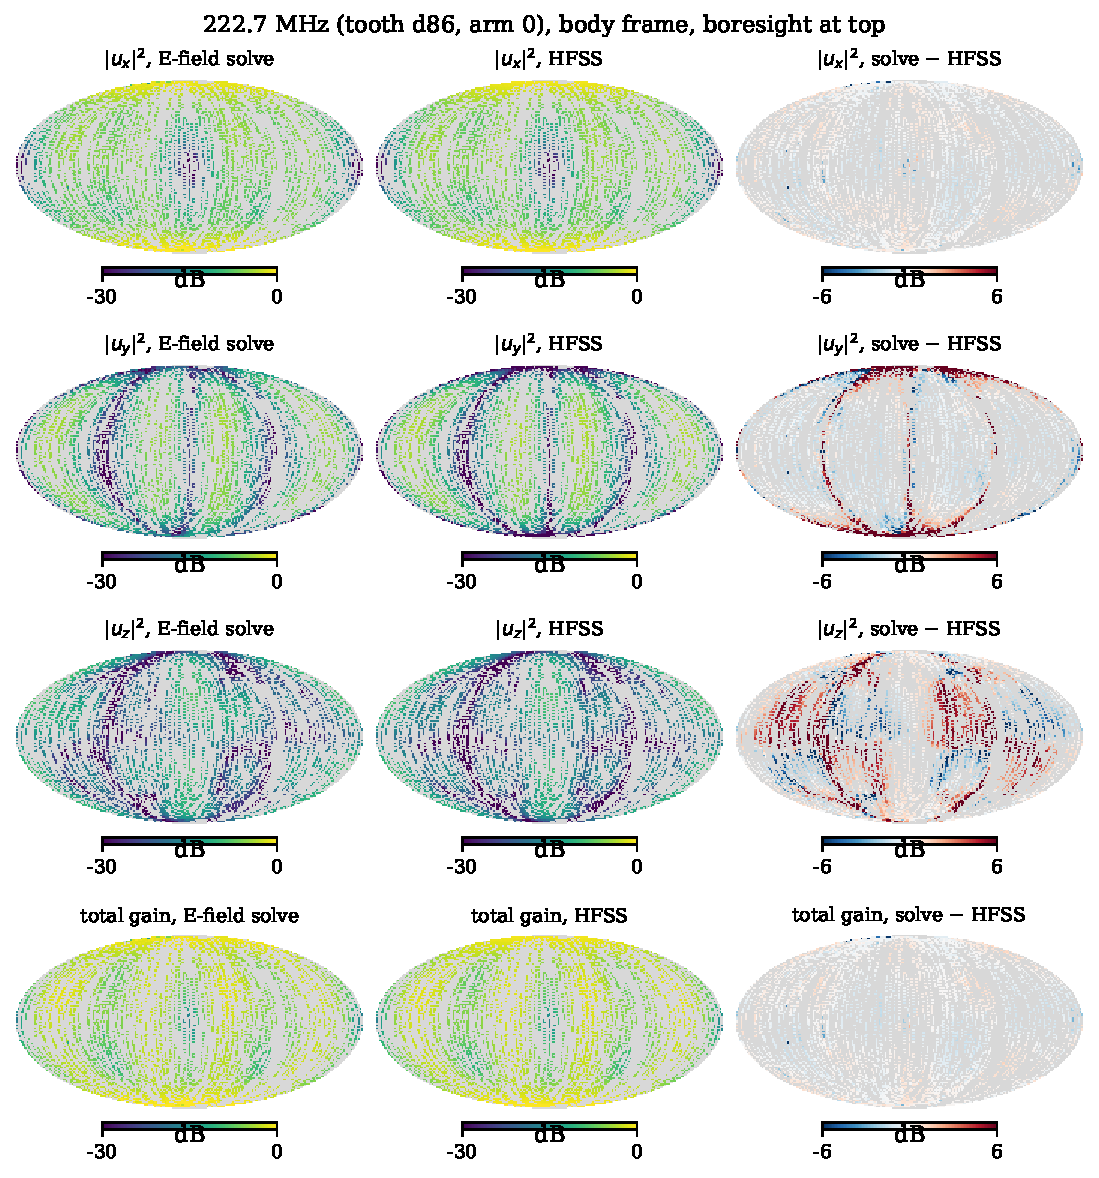
\includegraphics[width=0.92\textwidth]{figures/maps_d86.pdf}
\caption{As Fig.~\ref{fig:mapsA} at 222.7\,MHz; \mapNpixC\ pixels; rms difference \mapRmsDbC\,dB.}
\label{fig:mapsC}
\end{figure*}

\section{Validation} \label{sec:validation}
\begin{table}[h]
\centering
\caption{What each test holds out and what it can show (right-handed v0013 geometry unless stated).}
\label{tab:tests}
\begin{tabular}{p{0.24\linewidth}p{0.34\linewidth}p{0.34\linewidth}}
\hline
test & result & caveat \\
\hline
leave-one-out & 0.970 & optimistic: neighbours from the same dwell are near-duplicates \\
split half by dwell & $y$ is the weakest component everywhere & a first version split even and odd
  integrations, pairing consecutive ones; fixed \\
held-out stripes (memo 005's split) & solve 0.151 against HFSS 0.083; 0.090 with the per-dwell phase removed
  (\S\ref{sec:phase}) & reaches only pixels near el $\approx0^\circ$ or $\pm180^\circ$, $\sim$15\% of samples \\
single-visit pixels & reproduced to $10^{-14}$ & by construction; tests nothing \\
dwell repeatability (left-handed) & Table~\ref{tab:repeat} & \S\ref{sec:nulls} \\
\hline
\end{tabular}
\end{table}

\subsection{Noise or systematics at the nulls} \label{sec:nulls}
The $y$ and $z$ difference maps (Figs.~\ref{fig:mapsA}--\ref{fig:mapsC}) are worst along each component's
nulls. Three things can cause that:
\begin{itemize}
\item \textbf{Noise.} The solve gives all three components similar absolute errors, so a component far below
  $x$ drowns first.
\item \textbf{Leakage of $x$.} An error in the geometry, the transmitter polarization or $g$ rotates a little of
  $x$ into $y$ and $z$: a $1^\circ$ error leaks at about $-35$\,dB, $5^\circ$ at about $-21$\,dB. Such leakage
  changes with the roll at which a pixel is seen.
\item \textbf{HFSS's ideal nulls.} The real box, mast and cables probably fill nulls that HFSS keeps deep.
\end{itemize}
Pixels seen in two or more dwells separate the first two from the third. Each dwell is solved on its own and
compared with the other dwell and with HFSS. The comparison uses component powers $|u_k|^2$, which a common
per-dwell phase cannot change, on one real scale per tooth (as the maps), divided by HFSS's total power at the
pixel. Noise and roll-dependent leakage differ between dwells; an error that depends only on the body-frame
direction repeats. Pixels are binned by the component's share of HFSS's total power there, a measure of how
deep in its null it is (Table~\ref{tab:repeat}).

\begin{table}[h]
\centering
\caption{rms differences in units of the pixel's total HFSS power, over all teeth. Dwell vs dwell is divided by
  $\sqrt2$, so both columns are the error of one dwell. 6517 and 9066 pixel--tooth pairs have two or more dwells;
  the tilt changes which pixels are revisited.}
\label{tab:repeat}
\begin{tabular}{lcccc}
\hline
 & \multicolumn{2}{c}{left-handed, no tilt} & \multicolumn{2}{c}{left-handed, tilt $+4.7^\circ$} \\
component, HFSS share & dwell vs dwell & dwell vs HFSS & dwell vs dwell & dwell vs HFSS \\
\hline
$|u_y|^2$, $<1\%$    & 0.0071 & 0.0184 & 0.0066 & 0.0129 \\
$|u_y|^2$, 1--10\%   & 0.0356 & 0.0391 & 0.0143 & 0.0259 \\
$|u_y|^2$, $>10\%$   & 0.0912 & 0.0889 & 0.0536 & 0.0811 \\
$|u_z|^2$, $<1\%$    & 0.0070 & 0.0104 & 0.0033 & 0.0062 \\
$|u_z|^2$, 1--10\%   & 0.0136 & 0.0224 & 0.0096 & 0.0158 \\
$|u_x|^2$, $>10\%$   & 0.0768 & 0.0958 & 0.0657 & 0.0879 \\
\hline
\end{tabular}
\end{table}

\begin{itemize}
\item \textbf{In the nulls the error is mostly not noise.} With the tilt, a dwell differs from HFSS by about
  twice what it differs from another dwell: for share $<1\%$, $y$ 0.0129 against 0.0066 and $z$ 0.0062 against
  0.0033. About 74\% ($y$) and 71\% ($z$) of the variance against HFSS repeats between dwells. Noise is at most
  the dwell-to-dwell value, under 1\% of the total power.
\item \textbf{The tilt removed roll-dependent leakage.} Without it, $y$'s dwell-to-dwell scatter is 0.036 (share
  1--10\%) and 0.091 ($>10\%$); with it, 0.014 and 0.054. Without the tilt, the $y$ and $z$ disagreement between
  two dwells also tracks their roll difference (Spearman $-0.54$); with it the dependence nearly vanishes
  ($+0.10$). Which roll differences occur depends on where on the sky the revisits fall, so this is supporting
  evidence, not proof.
\item \textbf{What remains depends only on direction.} It is either the real antenna's nulls differing from
  HFSS's, or a geometry error that depends only on direction (the elevation zero, the positions). This test
  cannot tell them apart.
\item \textbf{It is small in total power.} Where $y$ or $z$ is off by more than 3\,dB, that component is a
  median 0.05--1.5\% of the pixel's total power, so the total gain agrees to within 3\,dB on all but 0.1--0.3\%
  of pixels. The total gain therefore tests mainly $x$; the per-component correlations and this table test $y$
  and $z$.
\end{itemize}

\section{The axle tilt and the handedness in the HFSS-free test} \label{sec:tilt}
An HFSS-free consistency test predicts each integration from other dwells within $1^\circ$ (Gaussian kernel,
$|\Delta t|>30$\,s) and scores the pooled error, refitting $g$ at every trial geometry. A rigid tilt of the mount
and a shift of the transmitter are degenerate, until memo 002's survey bounds the transmitter to 0.1\,m. Then
the tilt $\tau_1$ of the elevation axle, in $R=R_z(\psi)\,R_y(\tau_1)\,R_x(\mathrm{el})\,R_z(\mathrm{az})$,
becomes measurable (Fig.~\ref{fig:tilt}).
\begin{itemize}
\item \textbf{The data alone do not choose the handedness:} the best consistency scores tie (0.1625 against
  0.1629). Memo 003 settles it from the azimuth IMU and two photographs.
\item \textbf{The tilt's sign flips with the handedness.} Left-handed: consistency prefers $+1.3$ to $+4^\circ$,
  the HFSS held-out rms \tiltHfssL$^\circ$, and the v0016 fit $+4.7^\circ$, between the two. The elevation IMU
  reads $+5.9^\circ$, but its along-axle bias cannot be calibrated.
\item \textbf{HFSS asks for 2--4$^\circ$ more tilt than the data alone}, in both conventions. Part of what HFSS
  calls tilt may be beam difference.
\end{itemize}

\begin{figure*}[t]
\centering
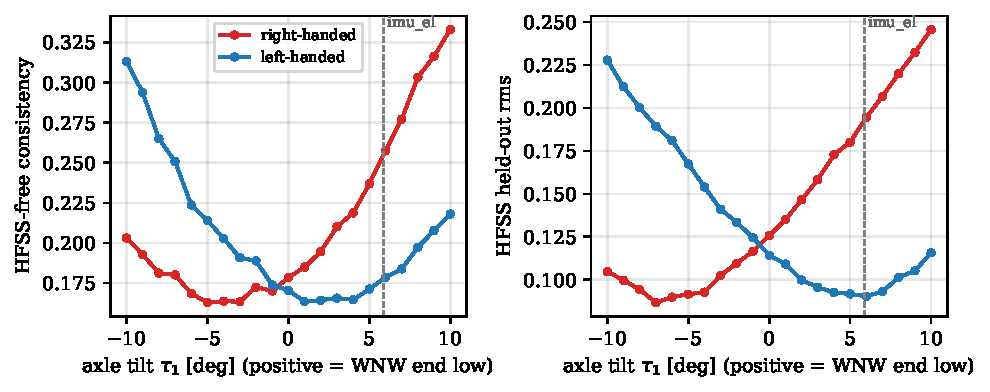
\includegraphics[width=\textwidth]{figures/tilt_scan.pdf}
\caption{Left: HFSS-free consistency (mean of even and odd teeth) against axle tilt. Right: HFSS held-out stripe
  rms, azimuth offset and $\alpha$ refitted per tilt. Red right-handed, blue left-handed azimuth; v0005
  posterior-mean positions; $g$ refitted at every tilt. Dashed: the elevation IMU's along-axle reading.}
\label{fig:tilt}
\end{figure*}

\section{Error budget against HFSS} \label{sec:budget}
Figure~\ref{fig:budget} adds physical terms to the HFSS power model one at a time and scores the held-out
stripes. It was computed under the right-handed azimuth, before memo 003's decision, and has not been redone;
the conclusion it supports, that the mount dominates the difference from HFSS, is what Fig.~\ref{fig:scores}
now shows directly. From the survey-only geometry, the shares in quadrature are geometry 0.086--0.096,
transmitter polarization 0.034--0.035, white noise 0.052, and a remainder (beam plus anything unmodelled, an
upper bound) of 0.062--0.074. The polarization term is arm-differential: the arms rotate oppositely as if
non-orthogonal by $\approx2.5^\circ$ below 205\,MHz and $\approx7^\circ$ above.

\begin{figure}[t]
\centering
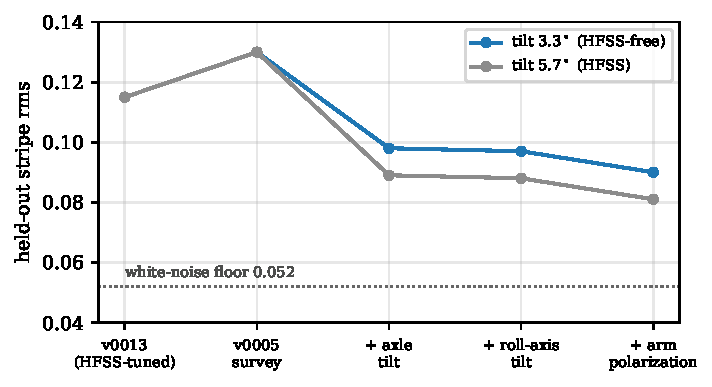
\includegraphics[width=\linewidth]{figures/error_budget.pdf}
\caption{Median held-out stripe rms over 29 teeth as physical terms are added to the HFSS model (right-handed
  azimuth). The v0013 start is low because its corrections were fitted to HFSS.}
\label{fig:budget}
\end{figure}

\section{The per-dwell common phase} \label{sec:phase}
Integrations a second apart, in nearly the same direction, agree to $2^\circ$ and 0.7\%. Visits a revolution
later (1--5\,min) differ by 3\% in amplitude but by $\sim56^\circ$ in phase, by the same amount in every tooth
($\pm5^\circ$). Over 172--227\,MHz a constant phase and a delay are nearly degenerate, and per-integration delays
were noise ($\pm1$\,ns), so the jump is treated as a phase.

A self-calibration (\texttt{vector\_beam.self\_calibrate\_phase}) fits one phase per block of 20 integrations to
other dwells' predictions. It transfers across halves of the band (held-out stripe rms 0.151 to 0.090, better on
29 of 29 teeth, with the phase from the other half), so it is not fitting noise. But a block that shares no
pixel with another dwell has no phase: only 4200 of 6810 integrations are calibrated, and a self-calibrated map
loses about 45\% of its pixels. Filling those phases would put an assumed phase on unmeasured data. The
self-calibration is therefore not used; its block phases serve below only as a diagnostic of the jumps.

\section{The cause of the phase jumps} \label{sec:jumps}
\begin{itemize}
\item \textbf{Not the lever arm or flexure} (memo 003 \S7): those depend only on pointing and are absorbed by the
  per-pixel beam.
\item \textbf{Not a steady drift:} the block phase averages $-0.8^\circ\,\mathrm{min}^{-1}$, against
  $+19^\circ\,\mathrm{min}^{-1}$ for memo 003's $+8.1\,\mathrm{cm\,min}^{-1}$; it wanders.
\item \textbf{Partly path-like:} the block phases from the two halves of the band correlate at 0.96, with a
  high/low ratio of $1.065\pm0.028$ against 1.153 for a path and 1.000 for a constant phase
  (Fig.~\ref{fig:jumps}, top).
\item \textbf{Not the elevation under-travel or the azimuth steps:} no correlation with jump size
  ($|r|<0.13$); blocks with an azimuth step $8.0^\circ$ against $9.8^\circ$ ($p=0.27$).
\item \textbf{Associated with rocking along the axle:} the along-axle tilt's range triples in minutes 20--40, and
  jump size rises with in-block rocking from $5.8^\circ$ to $15.8^\circ$ (lowest to highest quarter; $r=+0.26$,
  $p=0.003$). Two sharp excursions in the tilt, at minutes 28--29 and 33, coincide with the largest block-phase
  excursions ($\sim120^\circ$ and $\sim80^\circ$). Whether they are real motion is not checked.
\item \textbf{But not through pointing:} feeding the measured tilt into the geometry does not shrink the jumps
  ($9.7^\circ$ to $10.8^\circ$, $p=0.14$). Cables flexing, something on the box moving, or wind remain.
\end{itemize}

\begin{figure*}[t]
\centering
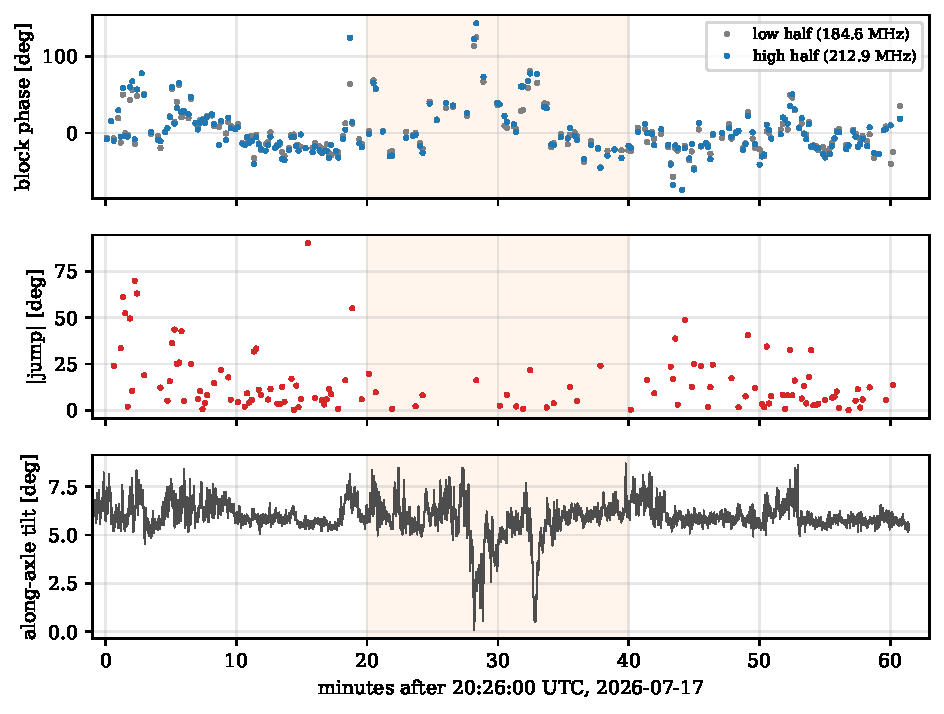
\includegraphics[width=\textwidth]{figures/phase_jumps.pdf}
\caption{Top: block phase from the low and high halves of the band. Middle: size of the jump between consecutive
  blocks. Bottom: box-air's tilt along the elevation axle from the raw imu\_el accelerometer. Shaded: minutes
  20--40, where the box rocks most. Right-handed geometry.}
\label{fig:jumps}
\end{figure*}

\section{Open questions} \label{sec:open}
\begin{itemize}
\item The direction-only residual at the nulls (\S\ref{sec:nulls}): real beam difference or remaining geometry.
\item The v0016 fit's remaining geometry corrections, not applied here.
\item The arm-differential transmitter polarization; memo 003's unexplained $10.3^\circ$ arm offset may be
  related.
\item The physical cause of the phase jumps: cable routing and wind data from the field; whether the two tilt
  excursions are real.
\item The crosses' three-point comb subtraction against the autos' DPSS bandpass.
\end{itemize}

\appendix
\section{Reproducing this memo} \label{app:repro}
Code: \texttt{eigsep\_data.beam\_mapping.vector\_beam} (EIGSEP/eigsep\_data main); the mount uses the
package's \texttt{TxGeometryModel} with \texttt{axle\_tilt\_deg} and \texttt{AZ\_SENSE}. Inputs: the raw files
\texttt{deployment5\_filtered/corr\_20260717\_*.h5}; pointing table v3 with the azimuth multiplied by
\texttt{AZ\_SENSE} as in v5; HFSS \texttt{bowtie\_beam.npz}. The driver scripts are in EIGSEP/data-analysis
\texttt{notebooks/dominic/vector\_beam/memo\_efield/}: \texttt{compute\_beams.py} (scores and maps),
\texttt{dwell\_repeatability.py}, \texttt{count\_auto\_pixels.py} and \texttt{make\_figures.py}, which writes
every figure and \texttt{values.tex}. The tilt scan, error budget and phase-jump analyses are in its
\texttt{supporting/} directory, as run under the right-handed convention.

\end{document}
